%\documentclass[a4paper]{book}


%%%%%%%%%% Various Packages %%%%%%%%%
\usepackage[english]{babel}
\usepackage[latin1]{inputenc}
\usepackage[numbers]{natbib}
\usepackage{verbatim} %% For Comment enviroment
\usepackage{lastpage}  % gives lastpage commando
\usepackage{algorithm}  %%% Algorithm Eviroment
\usepackage{algorithmic}  %%% Algorithm Eviroment
\usepackage{amsmath,amsfonts,amssymb,amsthm} % Math Paths
\usepackage{fancyhdr} % For headers
\usepackage{xifthen}% provides \isempty test and ifthen else 
\usepackage[absolute]{textpos} %used on the frontpage for the picture.
%%%%%%%%%%%%%%%%%%%%%%%%%%%%%%

%%%%%%% Protect against orhpans and widows %%%%%%%%%
\widowpenalty=300
\clubpenalty=300
%%%%%%%%%%%%%%%%%%%%%%%%%%%%%%%



%%%%%% Depracted  %%%%%%%%
%\usepackage{en-bib}  % anyone who knows this?
%\usepackage{en-bib}  % anyone who knows this?
%%%%%%%%%%%%%%%%%%%%


%%%%%%%%% Make links work %%%%%%%%%%
\usepackage[pdfborder={0 0 0 0}, backref=section]{hyperref}
%\usepackage[a4paper, bookmarks=true, bookmarksopen=true, bookmarksnumbered=true, pdfborder={0 0 0 0}, colorlinks=true, breaklinks=true, backref=section]{hyperref}
%%%%%%%%%%%%%%%%%%%%%%%%%%%%%%


%%% something? useful? hopefully!
\usepackage[]{graphicx} %dvips
\usepackage[]{subfig}% Need to make several pictures in one float
\usepackage{wrapfig}% Enables us to wrap text around a figure
%%%%%%%%%%%%%%%%%%%%%%%%%%%%%


%%%%%% Prettier chapters %%%%%
%\usepackage[Lenny]{fncychap}%
%\usepackage[Sonny]{fncychap}%
\usepackage[Bjornstrup]{fncychap}%
%\usepackage[Conny]{fncychap}%
%\usepackage[Rejne]{fncychap}%
%\usepackage{xparse}%
%%%%%%%%%%%%%%%%%%%%



%\setcitestyle{numbers}

%%%% Bibliography %%%%%%
\bibliographystyle{plainnat}
%%%%%%%%%%%%%%%%%


%%%%%% Something something might be important  %%%%%%%%%
\setcounter{tocdepth}{1}
\linespread{1}
%%%%%%%%%%%%%%%%%%%%

%%%%%%%%% Depracted %%%%%%%%%%%
%\setlength{\marginparwidth}{10pt}
%\setlength{\textwidth}{400pt}
%\setlength{\textheight}{620pt}
%\setlength{\voffset}{0pt}
%\setlength{\hoffset}{0pt}
%\setlength{\topmargin}{0pt}
%\setlength{\headsep}{10pt}
%\setlength{\oddsidemargin}{50pt}
%\setlength{\evensidemargin}{10pt}
%%%%%%%%%%%%%%%%%%%%



%%%%%%%%%%%%  COMMANDS   %%%%%%%%%%%%%%%%%%%%%%%
%%%%%%%%%%%%%%%%%%%%%%%%%%%%%%%%%%%%%%%%%%%
%%%%%%%%%%%%%%%%%%%%%%%%%%%%%%%%%%%%%%%%%%%
%%%%%%%%%%%%%%%%%%%%%%%%%%%%%%%%%%%%%%%%%%%

%%%%%%%%%% Get commands defined Elsewhere %%%%%%%%%
% c = first letter capital
% cap = all capital
% i = italic
% b = bold
% ci = first letter cap and all italic.
 \newcommand{\theWord}{some}
\newcommand{\caseControl}[4]{%
  \ifthenelse{\equal{#3}{c}}% First letter capital
    {\renewcommand{\theWord}{\MakeUppercase{#1}#2}}% if #1 true
    {}% if #1 false
     \ifthenelse{\equal{#3}{ci}}% first letter cap and italic
    {\renewcommand{\theWord}{\textit{\MakeUppercase{#1}#2}}}% if #1 true
    {}% if #1 false
      \ifthenelse{\equal{#3}{ic}}%% first letter cap and italic
    {\renewcommand{\theWord}{\textit{\MakeUppercase{#1}#2}}}% if #1 true
    {}% if #1 false
      \ifthenelse{\equal{#3}{i}}%% italic
    {\renewcommand{\theWord}{\textit{#1#2}}}% if #1 true
    {}% if #1 false
     \ifthenelse{\equal{#3}{cap}}% all cap
    {\renewcommand{\theWord}{\MakeUppercase{#1#2}}}% if #1 true
    {}% if #1 false
       \ifthenelse{\isempty{#3}}% %if nothing is stated 
    {\renewcommand{\theWord}{#1#2}}% if #1 true
    {}% if #1 false 
    \ifthenelse{\equal{\theWord}{some}}% % Double check actually
    {\renewcommand{\theWord}{#1#2}}% if #1 true
    {}% if #1 false 
    %%%%%% Standard definitions of words %%%%%%
        \ifthenelse{\equal{#4}{i}}% 
    {\textit{\theWord}}% if #1 true  % Print it italic
    {}% if #1 false 
	    \ifthenelse{\equal{#4}{b}}% Print it in bold
    {\textbf{\theWord}}% if #1 true
    {}% if #1 false 
        \ifthenelse{\equal{#4}{u}}% print it underlinde (not working yet)
    {{\theWord}}% if #1 true
    {}% if #1 false 
       \ifthenelse{\isempty{#4}}%  If there is nothing stated here just print the shit. 
    {\theWord}% if #1 true
    {}% if #1 false    
    \renewcommand{\theWord}{some}%
  }
\newcommand{\myMonth}{Some}
\newcommand{\myDate}[3]{%
\ifthenelse{\equal{#2}{1}}%
{\renewcommand{\myMonth}{January}}{}%
\ifthenelse{\equal{#2}{2}}%
{\renewcommand{\myMonth}{February}}{}%
\ifthenelse{\equal{#2}{3}}%
{\renewcommand{\myMonth}{Marts}}{}%
\ifthenelse{\equal{#2}{4}}%
{\renewcommand{\myMonth}{April}}{}%
\ifthenelse{\equal{#2}{5}}%
{\renewcommand{\myMonth}{May}}{}%
\ifthenelse{\equal{#2}{6}}%
{\renewcommand{\myMonth}{June}}{}%
\ifthenelse{\equal{#2}{7}}%
{\renewcommand{\myMonth}{July}}{}%
\ifthenelse{\equal{#2}{8}}%
{\renewcommand{\myMonth}{August}}{}%
\ifthenelse{\equal{#2}{9}}%
{\renewcommand{\myMonth}{September}}{}%
\ifthenelse{\equal{#2}{10}}%    
{\renewcommand{\myMonth}{October}}{}%
\ifthenelse{\equal{#2}{11}}%
{\renewcommand{\myMonth}{November}}{}%
\ifthenelse{\equal{#2}{12}}%
{\renewcommand{\myMonth}{December}}{}%
\ifthenelse{\isempty{#1}}%
{\myMonth{} #3}%
{\myMonth{} #1, #3}}%
%% This is where we define words. 
%% The last parameter should be blank as standard, but you can add i,b,u. 

%% WORD LIST
%% This is where we define words. 
%% The last parameter should be blank as standard, but you can add i,b,u. 
\newcommand{\john}[1]{\caseControl{j}{ohn}{#1}{}}
\newcommand{\michael}[1]{\caseControl{M}{ikael}{#1}{}}
\newcommand{\rubik}[1]{\caseControl{R}{ubik's Cube}{#1}{}}
\newcommand{\facet}[1]{\caseControl{f}{acet}{#1}{}}
\newcommand{\facelet}[1]{\caseControl{f}{acelett}{#1}{}}
\newcommand{\cube}[1]{\caseControl{c}{ube}{#1}{}}
\newcommand{\cuber}[1]{\caseControl{c}{uber}{#1}{}}
\newcommand{\face}[1]{\caseControl{f}{ace}{#1}{}}
\newcommand{\cpiece}[1]{\caseControl{p}{iece}{#1}{}}
\newcommand{\twist}[1]{\caseControl{t}{wist}{#1}{}}
\newcommand{\turn}[1]{\caseControl{t}{urn}{#1}{}}
\newcommand{\rotate}[1]{\caseControl{r}{otate}{#1}{}}
\newcommand{\erno}[1]{\caseControl{E}{rn\"{o} Rubik}{#1}{}}
\newcommand{\mpuzzle}[1]{\caseControl{M}{agic Puzzle}{#1}{}}
\newcommand{\msquare}[1]{\caseControl{M}{agic Square}{#1}{}}
\newcommand{\mcube}[1]{\caseControl{M}{agic Cube}{#1}{}}
%%%%%%%%%%%%%%%%%%%%

%%%%  Makes the titles look nicer. i guess. Rasmus out. %%%%%%% Don't remove
%\usepackage{titlesec} \newcommand{\bigrule}{\titlerule[0.5mm]} \titleformat{\chapter}[display] {\bfseries\Huge} {  \vskip-2em 
 %\titlerule 
% \filright  \huge\chaptertitlename\ \vspace{5mm}  \huge\thechapter} {0mm} {\filright} [\vspace{3mm} \bigrule \vspace{-10mm}] %
%%%%%%%%%%%%%%%%%%%%%%%%%%%%

%%%%% Depracted %%%%%%%%%
\newcommand{\picturepath}[1]{input/pics/}


%%%%% Used to determine the highlight of the first word in the terminology %%%%%
\newcommand{\myTermHigh}[1]{\textbf{#1}: }
%%%%%%%%%%%%%%%%%%%%%%

%%%%%%%%% tops 'n' tails %%%%%%%%%%%%
\newcommand{\myTop}[1]{\vspace{-8mm}  \vspace{0mm} \textit{#1} \vspace{3.4mm} \hrule \vspace{3.4mm} }
%\newcommand{\myTop}[1]{ \vspace{3.4mm} \textit{#1} \  \\  \hrule \  \\}%
\newcommand{\myTail}[1]{ \vspace{3.4mm} \hrule \vspace{3.4mm} \textit{#1} }%

\newcommand{\emptyTop}[0]{\vspace{-6mm}}
%%%%%%%%%%%%%%%%%%%%%%%%%%%%

%%%%%%%%% Use this for caption text %%%%%%%%%%
\newcommand{\myCaption}[1]{\textit{\footnotesize #1} }
%\usepackage[bf]{caption}
%%%%%%%%%%%%%%%%%%%%%%%%%%%%

%%%%%%%% Bruges til skillekolonner og r\ae{}kker . Definerer tykkelsen. %%%%%%
\newcommand{\vrules}{{\vrule width 0.6pt}}
\newcommand{\hrules}{{\hrule height 1.2pt}}
%%%%%%%%%%%%%%%%%%%%%%%%%%%%%%%%%%%%%%%%%%%

%%%%%%%Commands for getting e.g. ``st'' lifted in 1st   %%%%%%%%%%%
\newcommand{\superscript}[1]{\ensuremath{^{\textrm{#1}}}}
\newcommand{\subscript}[1]{\ensuremath{_{\textrm{#1}}}}
\newcommand{\ths}[0]{\superscript{th}}
\newcommand{\st}[0]{\superscript{st}}
\newcommand{\nd}[0]{\superscript{nd}}
\newcommand{\rd}[0]{\superscript{rd}}
%%%%%%%%%%%%%%%%%%%%%%%%%%%%%%%%%%%%%%%%%%%


%%%%%%%%%% Moves %%%%%%%%%%
\newcommand{\m}[1]{\textbf{#1}}
\newcommand{\vr}[1]{$#1$}
%%%%%%%%%%%%



%%%%%%%%% Defining Theorem %%%%%%%%%%%
\theoremstyle{definition} \newtheorem{theorem}{Theorem}
%%%%%%%%%%%%%%%%%%%%%%%%%%%%%%%%%%%%%%%%%%%


%%%%%%%%% List Environments %%%%%%%%%%%
\usepackage{listings}
\usepackage{color}

\definecolor{gray95}{gray}{.95}
\definecolor{gray92}{gray}{.92}
\definecolor{gray75}{gray}{.75}
\definecolor{gray45}{gray}{.45}

\lstdefinestyle{sourceCode}
{ 
	numbers=none, 
	stepnumber=1,
	captionpos = b,  %bottom
	keywordstyle=\color[rgb]{0,0,1},
	commentstyle=\color[rgb]{0.133,0.545,0.133},
	stringstyle=\color[rgb]{0.627,0.126,0.941},
	backgroundcolor=\color{gray95},
	frame=lrtb,
	framerule=0.5pt,
	linewidth = \textwidth,
	tabsize=2,
	numberbychapter=true,
	basicstyle=\ttfamily\footnotesize,
	language=java,
	breaklines=true,
	showstringspaces=false,
}

\renewcommand{\lstlistingname}{Code snippet}%%Changing the caption to read ``Code snippet''
\renewcommand{\lstlistlistingname}{Code snippets}

%%%%%%%%%% To use with copy-paste:
\begin{comment}

\begin{lstlisting}[style=sourceCode, caption=\myCaption{<some caption>}, label=<some label>]
<the code>
	<more code, now with indent>
\end{lstlisting}

\end{comment}
%%%%%%%%%% To input file:
\begin{comment}

\lstinputlisting[style=sourceCode, caption=\myCaption{<some caption>}, label=<some label>]{<file name>}

\end{comment}


\documentclass{article}
\bibliographystyle{plainnat}
\usepackage[english]{babel}
\usepackage[latin1]{inputenc}
\usepackage[numbers]{natbib}
\usepackage[]{graphicx} %dvips
\usepackage[]{subfig}% Need to make several pictures in one float
\usepackage{verbatim} %% For Comment enviroment
\usepackage{lastpage}  % gives lastpage commando
\usepackage{algorithm}  %%% Algorithm Eviroment
\usepackage{algorithmic}  %%% Algorithm Eviroment
\usepackage{amsmath,amsfonts,amssymb,amsthm} % Math Paths
\usepackage{fancyhdr} % For headers
\usepackage{xifthen}% provides \isempty test and ifthen else 
\setcounter{tocdepth}{1}
\linespread{1}

\begin{document}

%Forside
\thispagestyle{empty}
\begin{center}        % Sentrerer teksten
  %Tittel
  \vspace{5mm}          % Vertikalt mellomrom
  \LARGE
  \textbf{The Rubik's Cube} \\
  \Large
  \vspace{5mm}
  \textbf{by} \\
  \vspace{5mm}
  %Forfatter
  \large
  \textbf{A215} \\
  %Avdeling for mekanikk
  \vspace{10mm}
  \Large
  {\bf{\textsl{Status Seminar}}} \\
   \vspace{2mm}
  %%%%%%%OLD%%%%%%{\bf{\textsl{CANDIDATUS SCIENTIARUM}}} \\
  {\bf{\textsl{}}} \\
  \vspace{5mm}
  {\large \textsl {}}\\
  
  
  \vspace{10mm}
  \centerline{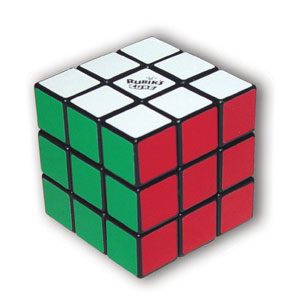
\includegraphics[width=4cm,height=4cm]{input/pics/rubiksCube}}
  \vspace{5mm}
  % \textsl{Mechanics Division, Department of Mathematics} \\
  \textsl{} \\
  \textsl{} \\
  %Maaned, aar
  \vspace{10mm}
  \large
  \textsl{Spring 2010} \\
  \vspace{5mm}
  \normalsize
  % \textsl{Avdeling for mekanikk, Matematisk institutt} \\
  \textsl{} \\
  \textsl{} \\
\end{center}

\ \pagebreak{}

\tableofcontents

\ \pagebreak{}
\section{Table of contents of the report}



\begin{figure}[hp]
	\centering
		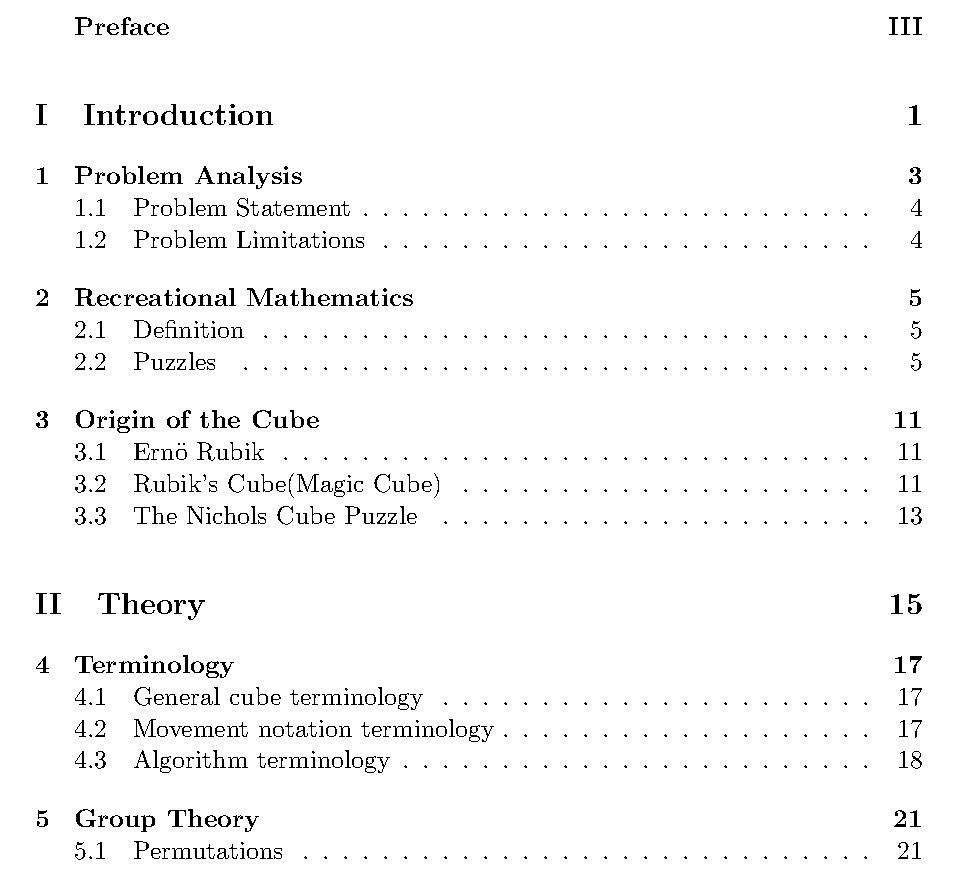
\includegraphics[scale = 0.7]{toc1.pdf}
		
		\label{fig:toc1}
\end{figure}
\begin{figure}
	\centering
		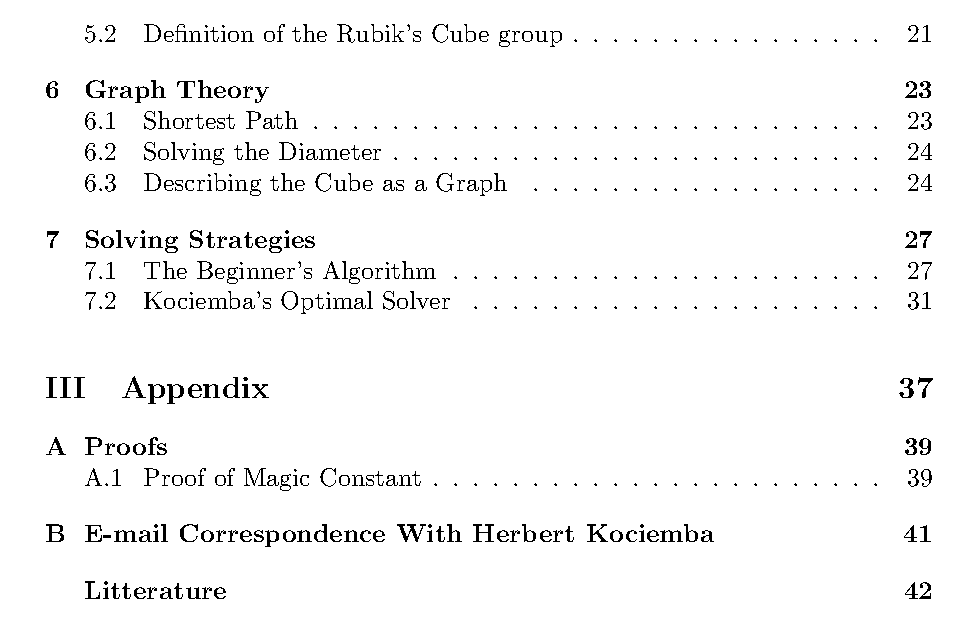
\includegraphics[scale = 0.7]{toc2.pdf}
	
	\label{fig:toc2}
\end{figure}




\ \pagebreak{}

\section{Problem Analysis}
Since 1977, when the Rubik's Cube was initially released for sale, the Rubik's Cube has frustrated, inspired and entertained many people. This 3x3x3 cube has so many possible settings that the solution can not just be guessed out of sheer luck. Because of this a community around solving the Rubik's Cube has emerged. The community is divided into two parts both concerning efficient solving -- one efficient time-wise and the other efficient twist-wise i.e. solving in the least amount of time and solving in the least amount of twists. 

The part concerning speed-wise efficiency, often referred to as speedcubing is the largest part of the community and the majority of the competitions held by the WCA\footnote{WCA, World Cube Association, is the official organization for Rubik's Cube related competitions.} revolve around speedcubing.

The first official competition was held in 1982 in Hungary and is regarded as the first World championship. Since 2002 there have been held annual world championships and plenty other events concerning speedcubing. 

The part of the community concerning twist-wise efficiency is much smaller than the speedsolving part. The majority of the research in the twist-wise efficient area is published as scientific articles explaining the algorithms. Even though competitions with the goal of the least amount of twists to solve the cube are held, many of the twist-wise efficient algorithms are not useful for human solving. These algorithms rely on computer power to look through a large amount of possibilities, which is not a viable option for a human competitor.

The ultimate goal for the twist-wise efficiency community is to find the God's algorithm, which is the algorithm that solves the cube in the absolute least amount of twists from any given position. A part of finding the God's algorithm is to find the amount of moves need to perform it. 
The upper bound of the Rubik's Cube is the maximum number of twists needed to solve an arbitrary Rubik's Cube.
The lower bound is the least number of twists required to solve the cube in the currently known worst case scenario. It is interesting to study this part of the Rubik's Cube community because it is currently moving, proving new upper bounds.

\subsection{Problem Statement}
What are the current upper and lower bound of the Rubik's Cube and how have they been proven? \\
\\
How can we create an application which can solve the Rubik's Cube?
\begin{itemize}
	\item Which algorithms can be used and which is the most efficient with respect to the number of twists?
\end{itemize}

\subsection{Problem Limitations}
Because the amount of different algorithms for Rubik's Cube solving, not every algorithm will be covered in this project.

The Rubik's Cube solving algorithm will be primarily for technical use, meaning that usability will not be in focus.

\section{Structure}
Our report is divided into four parts and an appendix. The four parts are Introduction, Theory, Implementation and Epilogue.
The contents of these parts are:
\begin{itemize}
	\item \textbf{Introduction:} Primarily contextual subjects are found within this part, such as recreational mathematics and origin of the cube. It is also in this part where the problem analysis is placed. This part is nearly completed.
	
	\item \textbf{Theory:} This part presents the fundamental theory regarding the Rubik's Cube. A general terminology initializes this part and is followed by group and graph theory. A description of two different solving strategies, beginner's algorithm and kociemba's optimal solver. This part is halfway done. We are currently working on a chapter regarding the upper bound of the Rubik's Cube.
	
	\item \textbf{Implementation:} We have not begun work on this part jet, but we intend to include a description of how our implementation of the Rubik's Cube and at least one solving strategy. Which algorithms we will implement is not yet discussed.
	 Our implementation will be made in Java, since we are all familiar with this language.
	\item \textbf{Epilogue:} Work on this part will not be started until our implementation is completed. In this part we will include a discussion of our implementation and theory as well as a conclusion on our problem statement.
\end{itemize}



\section{Strategy for problem solving}

We will achieve our goal and solve our problem statement by examining and understanding the theory of the Rubik's Cube and then apply it in an actual implementation. 

\subsection{The work process}
The actual work is done in subgroups consisting of 2-3 group members.  The subgroups have relatively short termed deadlines. The deadlines are organized on our wall-calender. In order to achieve the best result the work of one group is not only corrected by the author group but by an other group as well. The groups change between tasks. 

\subsection{The wall calendar}
In order to manage our schedule and tasks we use a large wall calendar. This calendar works as a post-it wall as well. A task is described with a post-it and contains both the task and the names of the members responsible for the task. The post-it is then placed on the date of the deadline. See figure \ref{fig:wall}
\begin{figure}[hp]
	\centering
		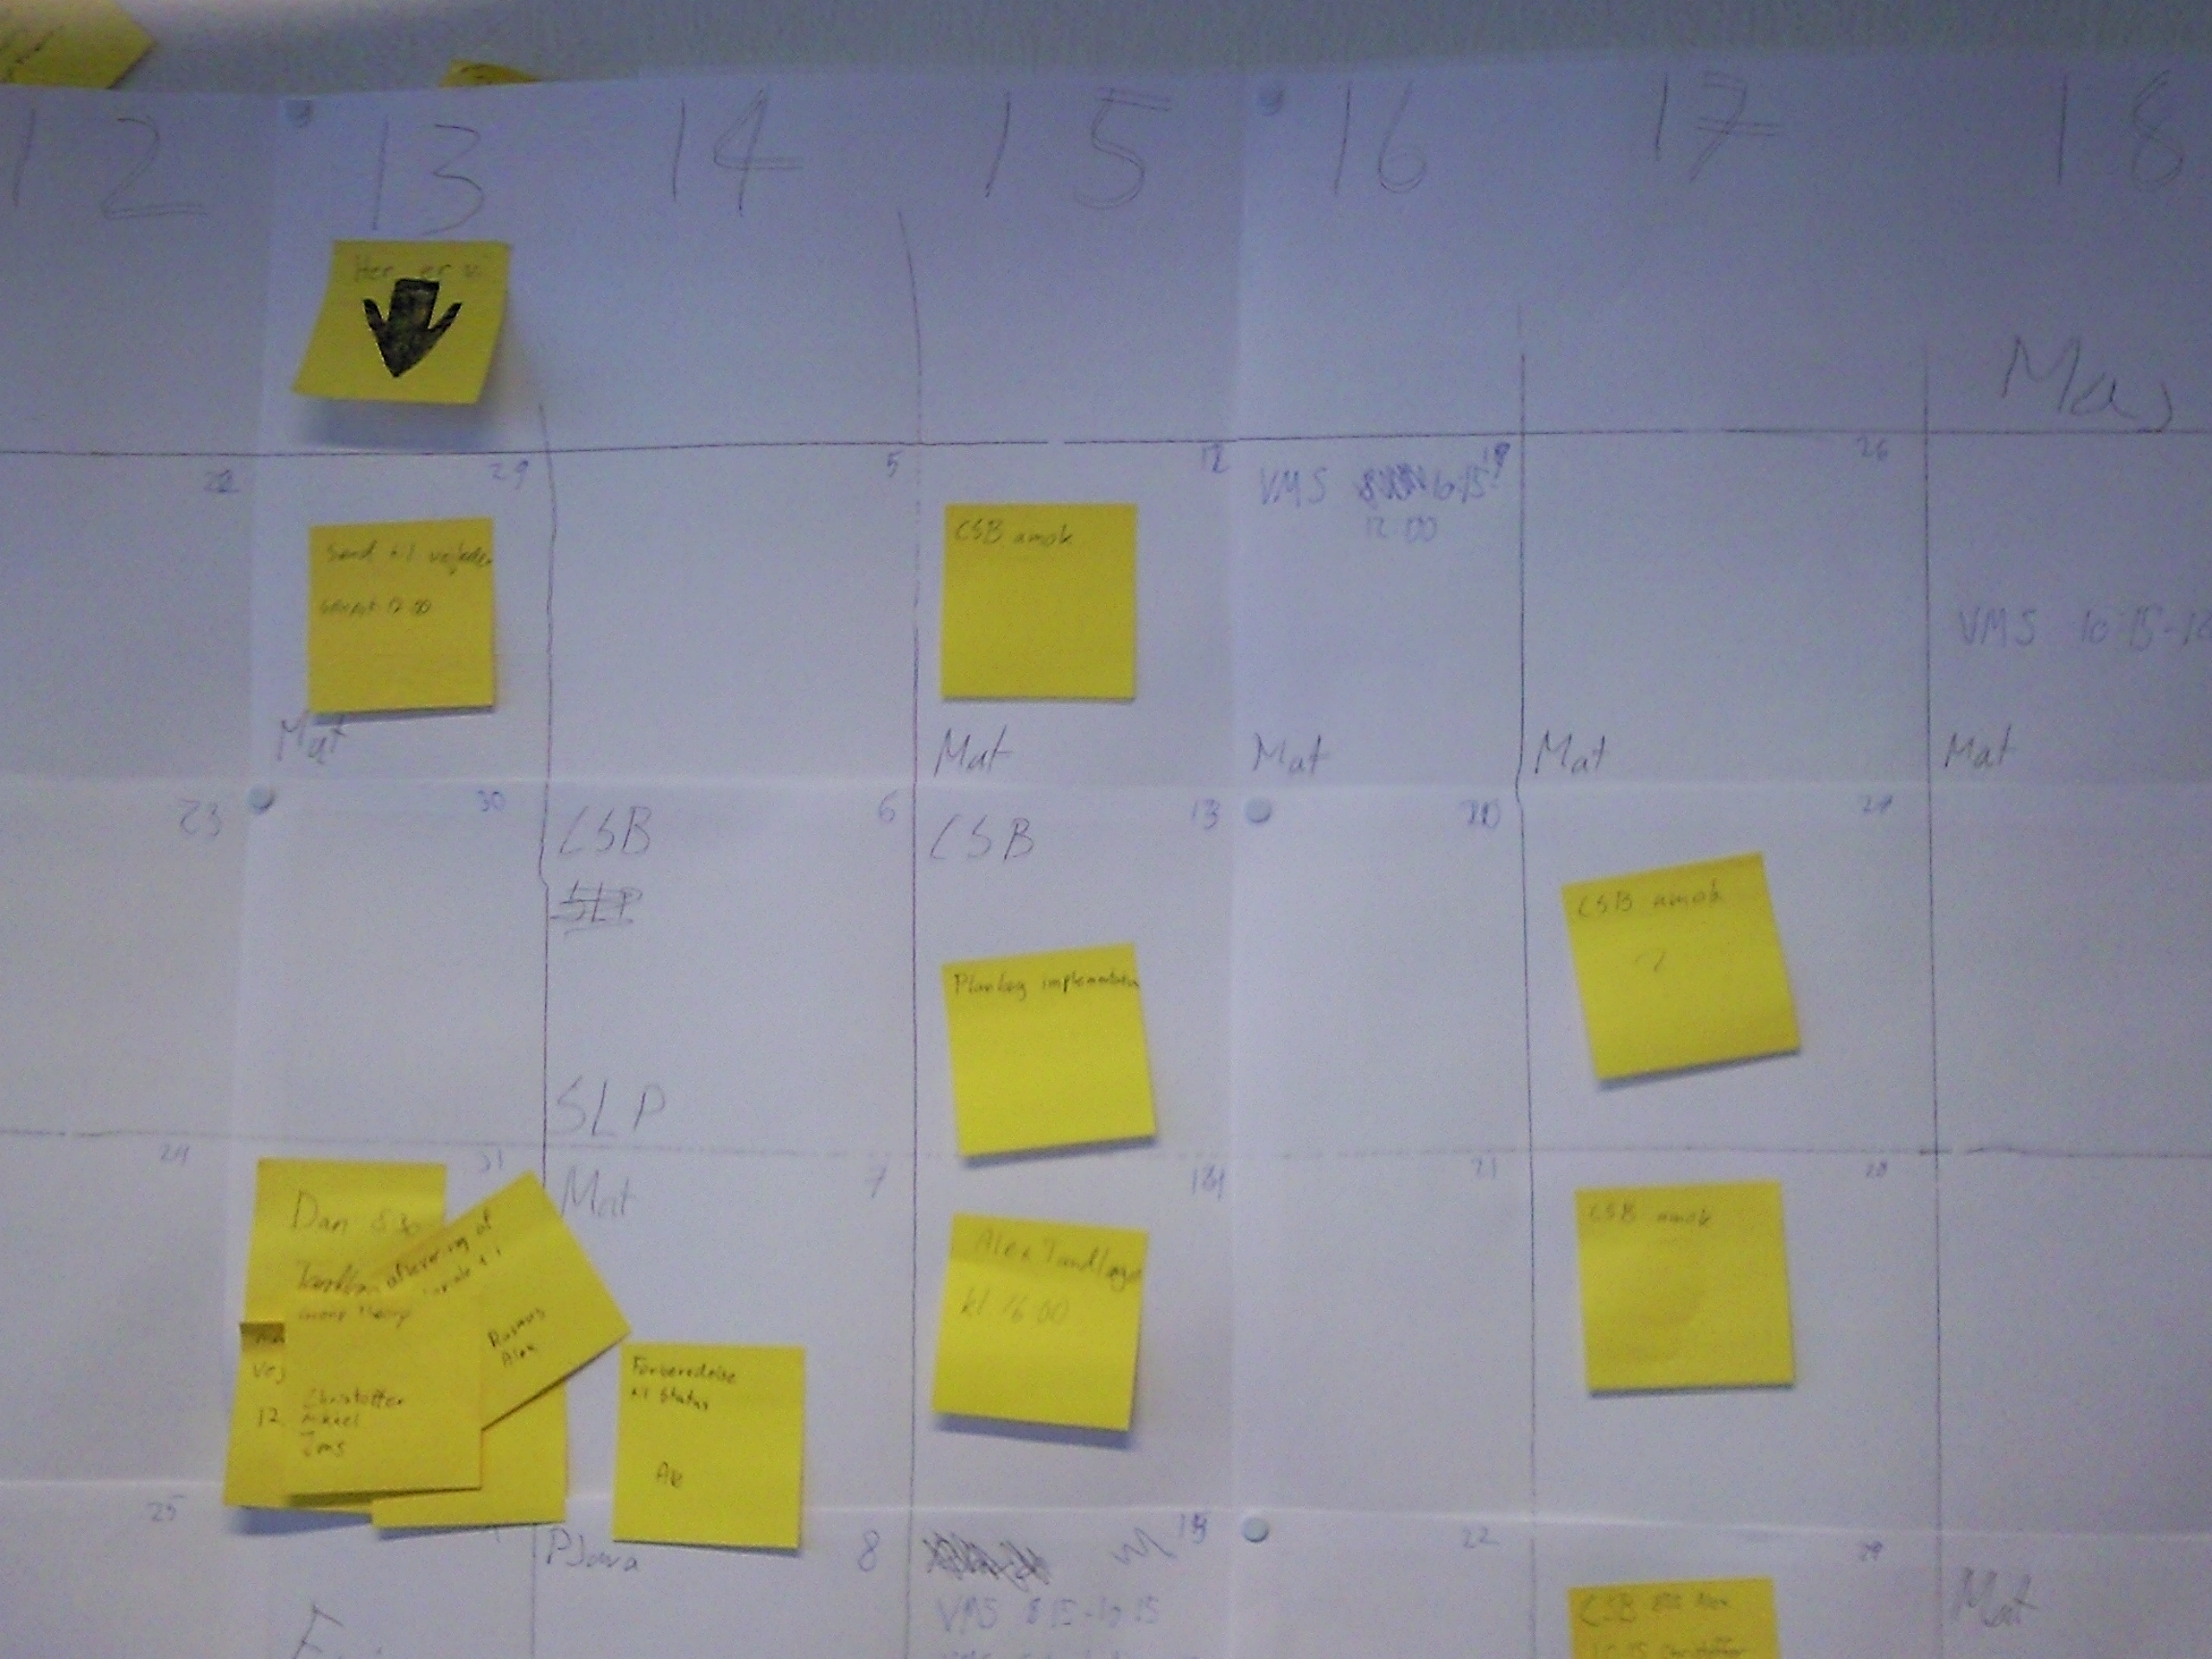
\includegraphics[scale = 0.1]{Billede0075.jpg}
		
		\label{fig:wall}
\end{figure}


\section{Resources}
We have taken email contact with Mr. Herbert Kociemba who is the author of one of the solving algorithms. We expect to use this contact to achieve more knowledge of his algorithm.

Every group member has a PC except for Rasmus who has a Mac. We have used these computers to work on our report and we will use them to write our implementation.

\section{Time plan}
Our current time plan is listed below. 
\begin{itemize}
	\item \textbf{March 8th:} Start on the theoretical part.
	\item \textbf{April 13th:} Start on the implementation part.
	\item \textbf{April 15th:} Start programming. 
	\item \textbf{May 7th:} Report ready for proofreading.
	\item \textbf{May 25th:} Report ready for printing.
	\item \textbf{May 27th:} Hand in report.
	\item \textbf{May 28th:} Hand in process analysis.
\end{itemize}


\section{Process Analysis}
The work has been proceeding in a steady pace. The time plan works since no deadlines have been exceeded. The work on the theory part is going well and we estimate that the date for the beginning work on the implementation will be as first planned. 

For the social parts we have not encountered any notable problems. We are in our group room from 8am till 3pm every day.

\end{document}